\subsection{LCD Display Port}

The \systemName~includes a liquid crystal display (LCD) port 
that is connected to the $16\times2$
character display on the \DEBoard~board. The display includes a memory for storing character
data. As indicated in Figure \ref{fig:LCD}$a$, the memory has a total capacity of
$40\times2$ characters. The first 16 characters stored in each row are visible on the
display, and the remaining 24 characters are not visible at any given time. Each location
in the memory can be accessed by combining the {\it x,y} coordinates into a 6-bit address
as depicted in Figure \ref{fig:LCD}$b$.  Using this scheme, the top and bottom rows of the 
display start at addresses (00)$_{16}$ and (40)$_{16}$, respectively, as we show in 
part $a$ of the figure.

The LCD display port automatically initializes and configures the $16\times2$ 
character display when the \systemName~is reset.
The programming interface for the LCD display port is illustrated in part $c$ of 
Figure \ref{fig:LCD}.  It includes an {\it Instruction} register that is used to control
the $16 \times 2$ character display, 
and a {\it Data} register that is used to send character data to the 
display. Data can be sent to the display as ASCII character codes, which are automatically 
converted by the $16 \times 2$ character display into bit patterns using a built-in font.

Some of the instructions supported by the $16 \times 2$ character
display are listed in Table \ref{tab:LCD}.
The first instruction, which is identified by the setting $b_7=1$, is used to set the location
of the cursor. The 6-bit {\it Address} field should be set using the values shown in
Figure \ref{fig:LCD}.  After the location of the cursor has been set, a character can 
be loaded into this location by writing its ASCII value into the {\it Data} register. 

\begin{figure}[h!]
   \begin{center}
       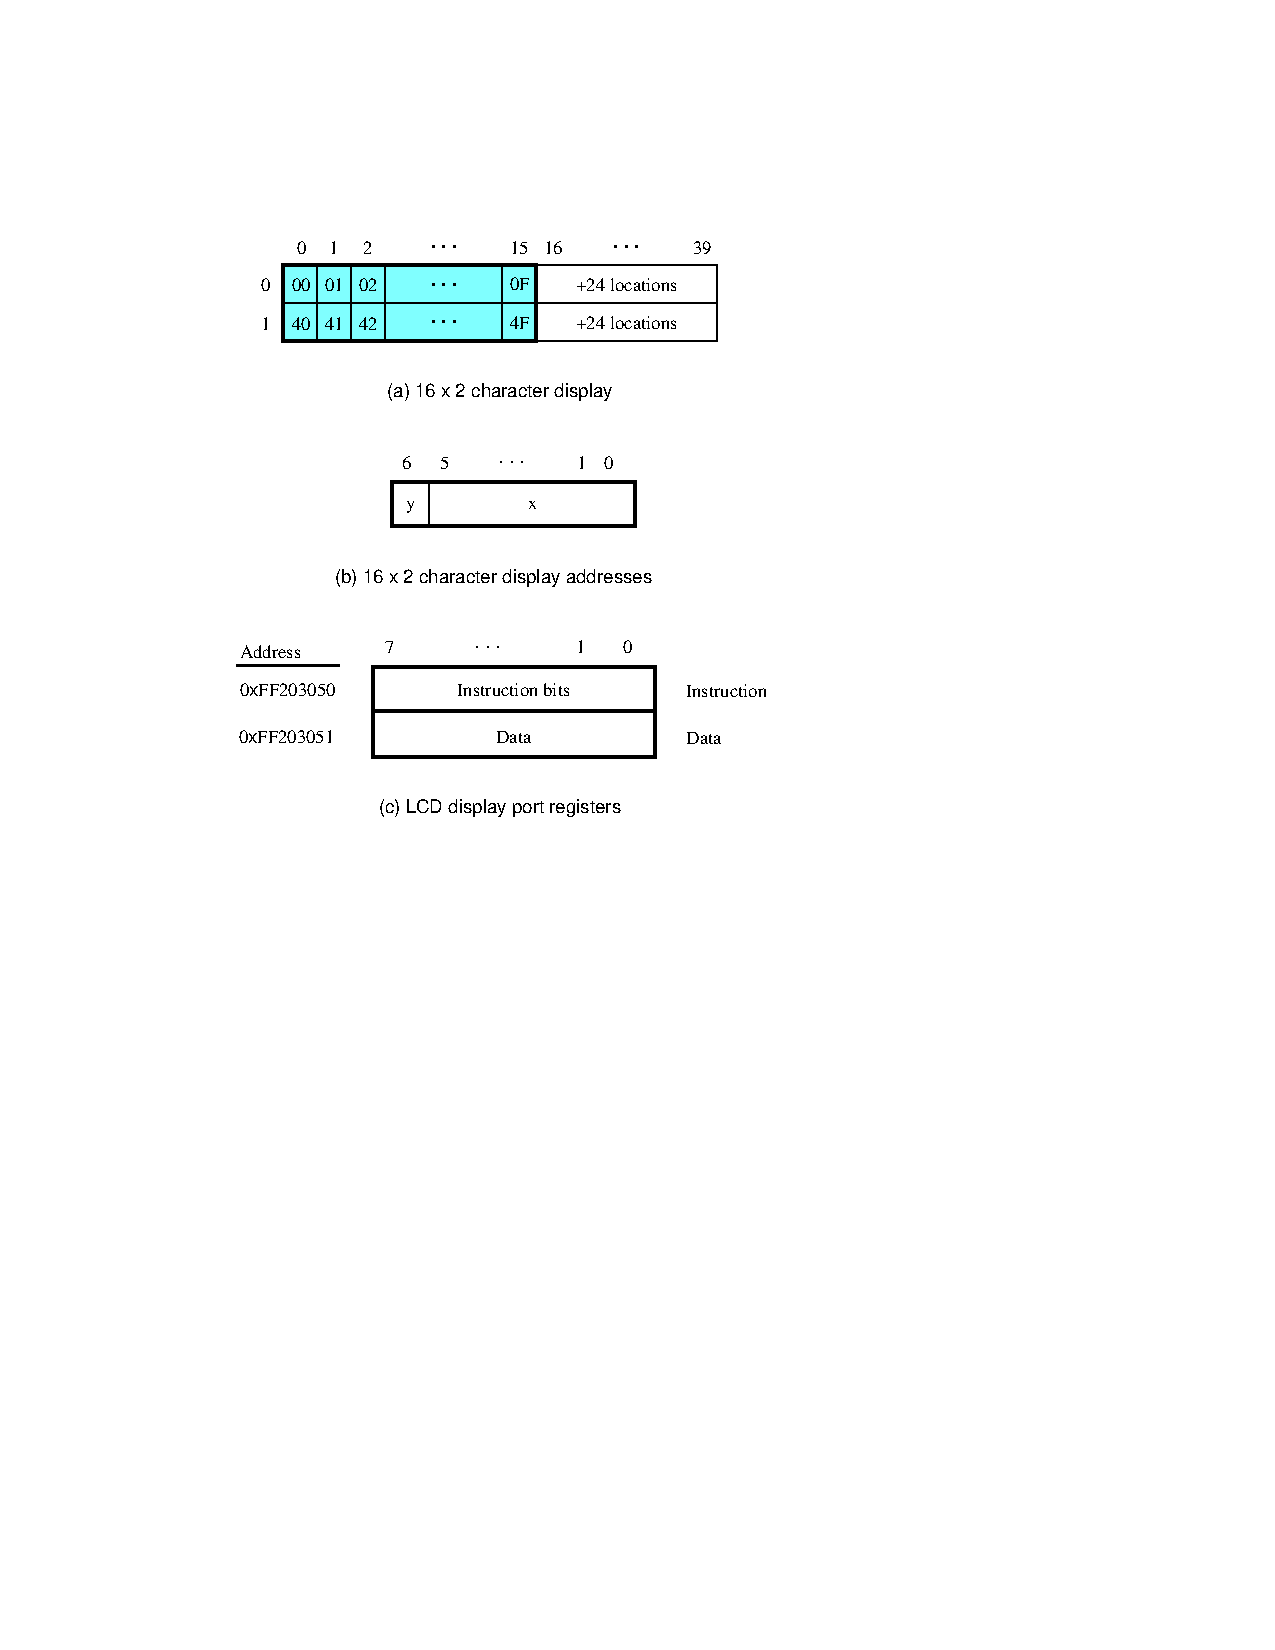
\includegraphics{\commonPath/../figs/Media_FPGA_LCD_Char.pdf}
   \end{center}
   \caption{LCD addresses and registers.}
	\label{fig:LCD}
\end{figure}

When data is written into the cursor location, the $16 \times 2$ character display 
automatically advances the cursor one position to the right. Multiple characters can 
be loaded into the display by writing each character in succession into the {\it Data} 
register. As we showed in Figure \ref{fig:LCD}, the $16 \times 2$ character display 
includes 40 locations in each row. When the cursor is
advanced past address (0F)$_{16}$ in the top row, the next 24 characters are stored in locations
that are not visible on the display. After 40 characters have been written into the top
row, the cursor advances to the bottom row at address (40)$_{16}$. At the end of the bottom row,
the cursor advances back to address (00)$_{16}$.

The $16 \times 2$ character display has the capability to shift its 
entire contents one position to the left
or right. As shown in Table \ref{tab:LCD}, the instruction for shifting left is
(18)$_{16}$ and the instruction for shifting right is (1C)$_{16}$. These instructions
cause both rows in the display to be shifted in parallel; when a character is shifted out
of one end of a row, it is rotated back into the other end of that same row. It is
possible to turn off the blinking cursor in the display by using the instruction (0C)$_{16}$, and
to turn it back on using (0F)$_{16}$. The display can be erased, and the cursor
location set to (00)$_{16}$, by using the instruction (01)$_{16}$.

\begin{table}[h]
    \begin{center}
    \begin{tabular}{l|ll}
            \textbf{Instruction} &
            \textbf{$b_7$} & \textbf{$b{6-0}$}
        \\\hline
            Set cursor location & 1 & {\it Address}
        \\
            Shift display left & 0 & 0011000
        \\
            Shift display right & 0 & 0011100
        \\
            Cursor off & 0 & 0001100
        \\
            Cursor blink on & 0 & 0001111
        \\
            Clear display & 0 & 0000001
        \\
    \end{tabular}
    \caption{LCD display instructions.}
	 \label{tab:LCD}
    \end{center}
\end{table}
